\documentclass{standalone}
\usepackage{tikz}
\usetikzlibrary{patterns, positioning}


\begin{document}
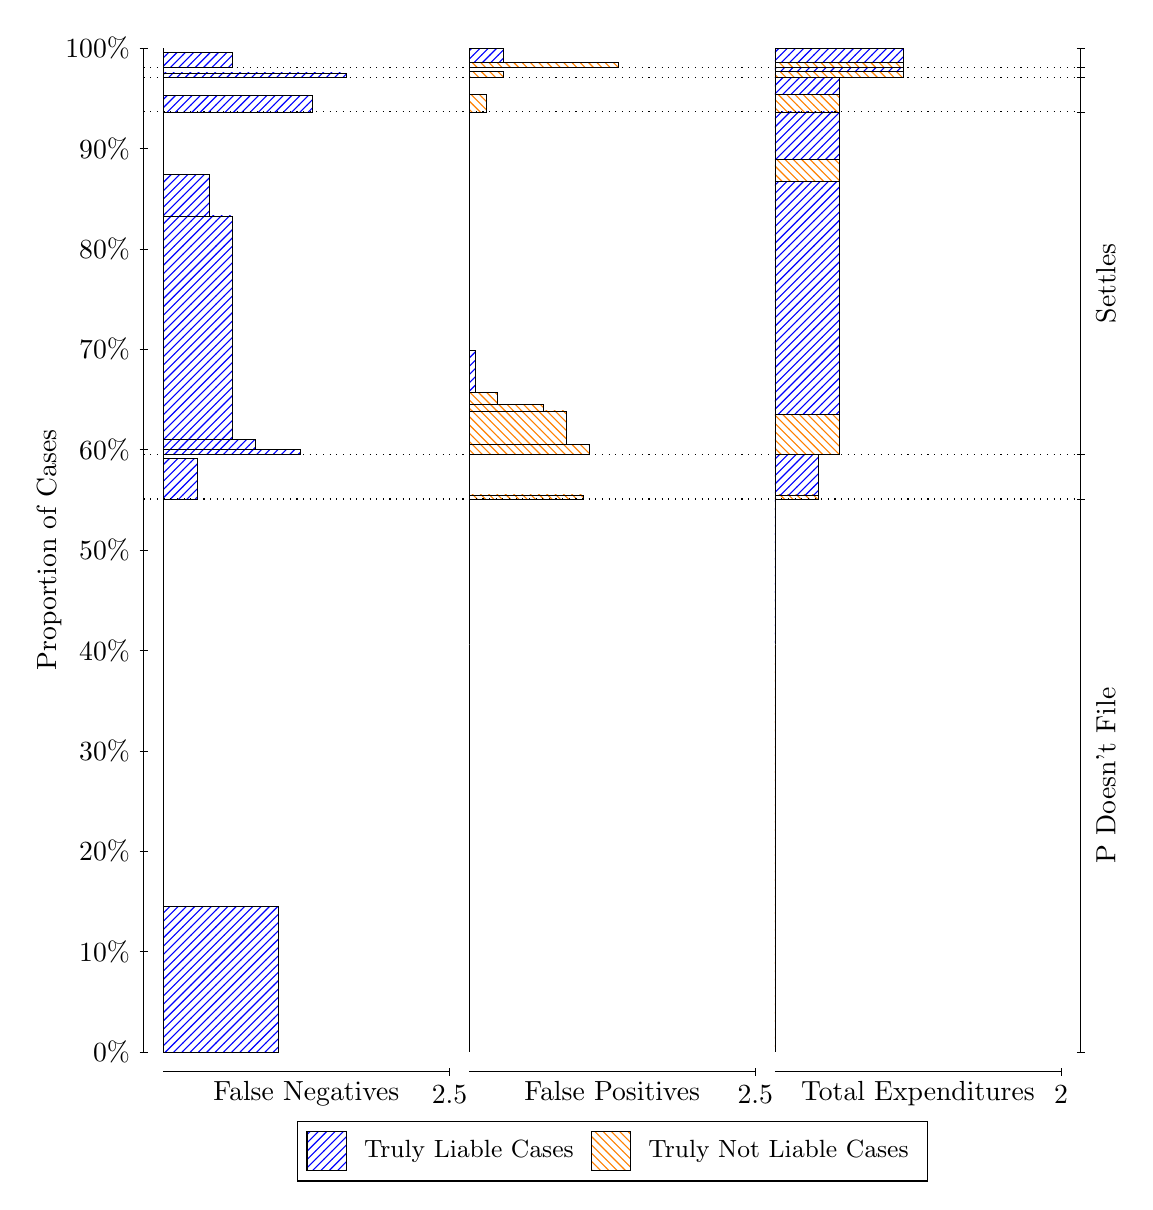
\begin{tikzpicture}
\draw[black, very thin] (1.5,1.75) -- (1.5,14.5);
\node[rotate=90, text=black, anchor=center] at (0.3, 8.125) {Proportion of Cases};
\draw[black, very thin] (1.45,1.75) -- (1.55,1.75);
\node[text=black, anchor=east] at (1.45, 1.75) {0\%};
\draw[black, very thin] (1.45,3.025) -- (1.55,3.025);
\node[text=black, anchor=east] at (1.45, 3.025) {10\%};
\draw[black, very thin] (1.45,4.3) -- (1.55,4.3);
\node[text=black, anchor=east] at (1.45, 4.3) {20\%};
\draw[black, very thin] (1.45,5.575) -- (1.55,5.575);
\node[text=black, anchor=east] at (1.45, 5.575) {30\%};
\draw[black, very thin] (1.45,6.85) -- (1.55,6.85);
\node[text=black, anchor=east] at (1.45, 6.85) {40\%};
\draw[black, very thin] (1.45,8.125) -- (1.55,8.125);
\node[text=black, anchor=east] at (1.45, 8.125) {50\%};
\draw[black, very thin] (1.45,9.4) -- (1.55,9.4);
\node[text=black, anchor=east] at (1.45, 9.4) {60\%};
\draw[black, very thin] (1.45,10.675) -- (1.55,10.675);
\node[text=black, anchor=east] at (1.45, 10.675) {70\%};
\draw[black, very thin] (1.45,11.95) -- (1.55,11.95);
\node[text=black, anchor=east] at (1.45, 11.95) {80\%};
\draw[black, very thin] (1.45,13.225) -- (1.55,13.225);
\node[text=black, anchor=east] at (1.45, 13.225) {90\%};
\draw[black, very thin] (1.45,14.5) -- (1.55,14.5);
\node[text=black, anchor=east] at (1.45, 14.5) {100\%};

\draw[black, very thin] (13.4,1.75) -- (13.4,14.5);
\draw[black, very thin] (13.35,1.75) -- (13.45,1.75);
\node[anchor=west] at (13.35, 1.75) {};
\draw[black, very thin] (13.35,8.7724) -- (13.45,8.7724);
\node[anchor=west] at (13.35, 8.7724) {};
\draw[black, very thin] (13.35,9.3378) -- (13.45,9.3378);
\node[anchor=west] at (13.35, 9.3378) {};
\draw[black, very thin] (13.35,13.689) -- (13.45,13.689);
\node[anchor=west] at (13.35, 13.689) {};
\draw[black, very thin] (13.35,14.127) -- (13.45,14.127);
\node[anchor=west] at (13.35, 14.127) {};
\draw[black, very thin] (13.35,14.258) -- (13.45,14.258);
\node[anchor=west] at (13.35, 14.258) {};
\draw[black, very thin] (13.35,14.5) -- (13.45,14.5);
\node[anchor=west] at (13.35, 14.5) {};

\draw[black, very thin, pattern color=blue, pattern=north east lines] (1.75,1.75) rectangle (3.2033,3.5955);
\draw[black, very thin, pattern color=orange, pattern=north west lines] (1.75,3.5955) rectangle (1.75,8.7724);
\draw[black, very thin, pattern color=blue, pattern=north east lines] (1.75,8.7724) rectangle (2.186,9.2849);
\draw[black, very thin, pattern color=orange, pattern=north west lines] (1.75,9.2849) rectangle (1.75,9.3378);
\draw[black, very thin, pattern color=blue, pattern=north east lines] (1.75,9.3378) rectangle (3.494,9.4068);
\draw[black, very thin, pattern color=blue, pattern=north east lines] (1.75,9.4068) rectangle (2.9127,9.5287);
\draw[black, very thin, pattern color=blue, pattern=north east lines] (1.75,9.5287) rectangle (2.622,12.367);
\draw[black, very thin, pattern color=blue, pattern=north east lines] (1.75,12.367) rectangle (2.3313,12.899);
\draw[black, very thin, pattern color=orange, pattern=north west lines] (1.75,12.899) rectangle (1.75,13.689);
\draw[black, very thin, pattern color=blue, pattern=north east lines] (1.75,13.689) rectangle (3.6393,13.902);
\draw[black, very thin, pattern color=orange, pattern=north west lines] (1.75,13.902) rectangle (1.75,14.127);
\draw[black, very thin, pattern color=blue, pattern=north east lines] (1.75,14.127) rectangle (4.0753,14.184);
\draw[black, very thin, pattern color=orange, pattern=north west lines] (1.75,14.184) rectangle (1.75,14.258);
\draw[black, very thin, pattern color=blue, pattern=north east lines] (1.75,14.258) rectangle (2.622,14.442);
\draw[black, very thin, pattern color=orange, pattern=north west lines] (1.75,14.442) rectangle (1.75,14.5);
\draw[black, very thin, pattern color=orange, pattern=north west lines] (5.6333,1.75) rectangle (5.6333,6.9269);
\draw[black, very thin, pattern color=blue, pattern=north east lines] (5.6333,6.9269) rectangle (5.6333,8.7724);
\draw[black, very thin, pattern color=orange, pattern=north west lines] (5.6333,8.7724) rectangle (7.0867,8.8254);
\draw[black, very thin, pattern color=blue, pattern=north east lines] (5.6333,8.8254) rectangle (5.6333,9.3378);
\draw[black, very thin, pattern color=orange, pattern=north west lines] (5.6333,9.3378) rectangle (7.1593,9.4633);
\draw[black, very thin, pattern color=orange, pattern=north west lines] (5.6333,9.4633) rectangle (6.8687,9.8918);
\draw[black, very thin, pattern color=orange, pattern=north west lines] (5.6333,9.8918) rectangle (6.578,9.9712);
\draw[black, very thin, pattern color=orange, pattern=north west lines] (5.6333,9.9712) rectangle (5.9967,10.127);
\draw[black, very thin, pattern color=blue, pattern=north east lines] (5.6333,10.127) rectangle (5.706,10.66);
\draw[black, very thin, pattern color=blue, pattern=north east lines] (5.6333,10.66) rectangle (5.6333,13.689);
\draw[black, very thin, pattern color=orange, pattern=north west lines] (5.6333,13.689) rectangle (5.8513,13.913);
\draw[black, very thin, pattern color=blue, pattern=north east lines] (5.6333,13.913) rectangle (5.6333,14.127);
\draw[black, very thin, pattern color=orange, pattern=north west lines] (5.6333,14.127) rectangle (6.0693,14.2);
\draw[black, very thin, pattern color=blue, pattern=north east lines] (5.6333,14.2) rectangle (5.6333,14.258);
\draw[black, very thin, pattern color=orange, pattern=north west lines] (5.6333,14.258) rectangle (7.5227,14.316);
\draw[black, very thin, pattern color=blue, pattern=north east lines] (5.6333,14.316) rectangle (6.0693,14.5);
\draw[black, very thin, pattern color=orange, pattern=north west lines] (9.5167,1.75) rectangle (9.5167,6.9269);
\draw[black, very thin, pattern color=blue, pattern=north east lines] (9.5167,6.9269) rectangle (9.5167,8.7724);
\draw[black, very thin, pattern color=orange, pattern=north west lines] (9.5167,8.7724) rectangle (10.062,8.8254);
\draw[black, very thin, pattern color=blue, pattern=north east lines] (9.5167,8.8254) rectangle (10.062,9.3378);
\draw[black, very thin, pattern color=orange, pattern=north west lines] (9.5167,9.3378) rectangle (10.334,9.8457);
\draw[black, very thin, pattern color=blue, pattern=north east lines] (9.5167,9.8457) rectangle (10.334,12.806);
\draw[black, very thin, pattern color=orange, pattern=north west lines] (9.5167,12.806) rectangle (10.334,13.087);
\draw[black, very thin, pattern color=blue, pattern=north east lines] (9.5167,13.087) rectangle (10.334,13.689);
\draw[black, very thin, pattern color=orange, pattern=north west lines] (9.5167,13.689) rectangle (10.334,13.913);
\draw[black, very thin, pattern color=blue, pattern=north east lines] (9.5167,13.913) rectangle (10.334,14.127);
\draw[black, very thin, pattern color=orange, pattern=north west lines] (9.5167,14.127) rectangle (11.152,14.2);
\draw[black, very thin, pattern color=blue, pattern=north east lines] (9.5167,14.2) rectangle (11.152,14.258);
\draw[black, very thin, pattern color=orange, pattern=north west lines] (9.5167,14.258) rectangle (11.152,14.316);
\draw[black, very thin, pattern color=blue, pattern=north east lines] (9.5167,14.316) rectangle (11.152,14.5);
\draw[black, dotted] (1.5,8.7724) -- (13.4,8.7724);
\draw[black, dotted] (1.5,9.3378) -- (13.4,9.3378);
\draw[black, dotted] (1.5,13.689) -- (13.4,13.689);
\draw[black, dotted] (1.5,14.127) -- (13.4,14.127);
\draw[black, dotted] (1.5,14.258) -- (13.4,14.258);
\draw[black, very thin] (1.75,1.5) -- (5.3833,1.5);
\node[text=black, anchor=north] at (3.5667, 1.5) {False Negatives};
\draw[black, very thin] (5.3833,1.45) -- (5.3833,1.55);
\node[text=black, anchor=north] at (5.3833, 1.45) {2.5};

\draw[black, very thin] (5.6333,1.5) -- (9.2667,1.5);
\node[text=black, anchor=north] at (7.45, 1.5) {False Positives};
\draw[black, very thin] (9.2667,1.45) -- (9.2667,1.55);
\node[text=black, anchor=north] at (9.2667, 1.45) {2.5};

\draw[black, very thin] (9.5167,1.5) -- (13.15,1.5);
\node[text=black, anchor=north] at (11.333, 1.5) {Total Expenditures};
\draw[black, very thin] (13.15,1.45) -- (13.15,1.55);
\node[text=black, anchor=north] at (13.15, 1.45) {2};

\node[text=black, centered, rotate=90] at (13.72, 5.2612) {P Doesn't File};

\node[text=black, centered, rotate=90] at (13.72, 11.513) {Settles};




\draw (7.449999999999999,1.5) node[draw=none] (baseCoordinate) {};
\begin{scope}[align=center]
        \matrix[scale=0.5, draw=black, below=0.5cm of baseCoordinate, nodes={draw}, column sep=0.1cm]{
            \node[rectangle, draw, minimum width=0.5cm, minimum height=0.5cm, pattern color=blue, pattern=north east lines] {}; &
            \node[draw=none, font=\small, text=black] (B) {Truly Liable Cases}; &
            \node[rectangle, draw, minimum width=0.5cm, minimum height=0.5cm, pattern color=orange, pattern=north west lines] {}; &
            \node[draw=none, font=\small, text=black] (B) {Truly Not Liable Cases}; \\
            };
\end{scope}

\end{tikzpicture}
\end{document}